\documentclass[twoside]{book}

% Packages required by doxygen
\usepackage{fixltx2e}
\usepackage{calc}
\usepackage{doxygen}
\usepackage[export]{adjustbox} % also loads graphicx
\usepackage{graphicx}
\usepackage[utf8]{inputenc}
\usepackage{makeidx}
\usepackage{multicol}
\usepackage{multirow}
\PassOptionsToPackage{warn}{textcomp}
\usepackage{textcomp}
\usepackage[nointegrals]{wasysym}
\usepackage[table]{xcolor}

% Font selection
\usepackage[T1]{fontenc}
\usepackage[scaled=.90]{helvet}
\usepackage{courier}
\usepackage{amssymb}
\usepackage{sectsty}
\renewcommand{\familydefault}{\sfdefault}
\allsectionsfont{%
  \fontseries{bc}\selectfont%
  \color{darkgray}%
}
\renewcommand{\DoxyLabelFont}{%
  \fontseries{bc}\selectfont%
  \color{darkgray}%
}
\newcommand{\+}{\discretionary{\mbox{\scriptsize$\hookleftarrow$}}{}{}}

% Page & text layout
\usepackage{geometry}
\geometry{%
  a4paper,%
  top=2.5cm,%
  bottom=2.5cm,%
  left=2.5cm,%
  right=2.5cm%
}
\tolerance=750
\hfuzz=15pt
\hbadness=750
\setlength{\emergencystretch}{15pt}
\setlength{\parindent}{0cm}
\setlength{\parskip}{3ex plus 2ex minus 2ex}
\makeatletter
\renewcommand{\paragraph}{%
  \@startsection{paragraph}{4}{0ex}{-1.0ex}{1.0ex}{%
    \normalfont\normalsize\bfseries\SS@parafont%
  }%
}
\renewcommand{\subparagraph}{%
  \@startsection{subparagraph}{5}{0ex}{-1.0ex}{1.0ex}{%
    \normalfont\normalsize\bfseries\SS@subparafont%
  }%
}
\makeatother

% Headers & footers
\usepackage{fancyhdr}
\pagestyle{fancyplain}
\fancyhead[LE]{\fancyplain{}{\bfseries\thepage}}
\fancyhead[CE]{\fancyplain{}{}}
\fancyhead[RE]{\fancyplain{}{\bfseries\leftmark}}
\fancyhead[LO]{\fancyplain{}{\bfseries\rightmark}}
\fancyhead[CO]{\fancyplain{}{}}
\fancyhead[RO]{\fancyplain{}{\bfseries\thepage}}
\fancyfoot[LE]{\fancyplain{}{}}
\fancyfoot[CE]{\fancyplain{}{}}
\fancyfoot[RE]{\fancyplain{}{\bfseries\scriptsize Generated by Doxygen }}
\fancyfoot[LO]{\fancyplain{}{\bfseries\scriptsize Generated by Doxygen }}
\fancyfoot[CO]{\fancyplain{}{}}
\fancyfoot[RO]{\fancyplain{}{}}
\renewcommand{\footrulewidth}{0.4pt}
\renewcommand{\chaptermark}[1]{%
  \markboth{#1}{}%
}
\renewcommand{\sectionmark}[1]{%
  \markright{\thesection\ #1}%
}

% Indices & bibliography
\usepackage{natbib}
\usepackage[titles]{tocloft}
\setcounter{tocdepth}{3}
\setcounter{secnumdepth}{5}
\makeindex

% Hyperlinks (required, but should be loaded last)
\usepackage{ifpdf}
\ifpdf
  \usepackage[pdftex,pagebackref=true]{hyperref}
\else
  \usepackage[ps2pdf,pagebackref=true]{hyperref}
\fi
\hypersetup{%
  colorlinks=true,%
  linkcolor=blue,%
  citecolor=blue,%
  unicode%
}

% Custom commands
\newcommand{\clearemptydoublepage}{%
  \newpage{\pagestyle{empty}\cleardoublepage}%
}

\usepackage{caption}
\captionsetup{labelsep=space,justification=centering,font={bf},singlelinecheck=off,skip=4pt,position=top}

%===== C O N T E N T S =====

\begin{document}

% Titlepage & ToC
\hypersetup{pageanchor=false,
             bookmarksnumbered=true,
             pdfencoding=unicode
            }
\pagenumbering{alph}
\begin{titlepage}
\vspace*{7cm}
\begin{center}%
{\Large Lab 4 }\\
\vspace*{1cm}
{\large Generated by Doxygen 1.8.13}\\
\end{center}
\end{titlepage}
\clearemptydoublepage
\pagenumbering{roman}
\tableofcontents
\clearemptydoublepage
\pagenumbering{arabic}
\hypersetup{pageanchor=true}

%--- Begin generated contents ---
\chapter{Class Index}
\section{Class List}
Here are the classes, structs, unions and interfaces with brief descriptions\+:\begin{DoxyCompactList}
\item\contentsline{section}{\hyperlink{structBalancedBinTree}{Balanced\+Bin\+Tree} }{\pageref{structBalancedBinTree}}{}
\item\contentsline{section}{\hyperlink{structBalancedBinTreeNode}{Balanced\+Bin\+Tree\+Node} }{\pageref{structBalancedBinTreeNode}}{}
\end{DoxyCompactList}

\chapter{File Index}
\section{File List}
Here is a list of all documented files with brief descriptions\+:\begin{DoxyCompactList}
\item\contentsline{section}{include/\hyperlink{heap_8h}{heap.\+h} \\*File containing the function definitions of a heap }{\pageref{heap_8h}}{}
\item\contentsline{section}{include/{\bfseries heap\+A\+D\+T.\+h} }{\pageref{heapADT_8h}}{}
\item\contentsline{section}{include/\hyperlink{hospital_8h}{hospital.\+h} \\*File containing the extra function for Assignment 3 }{\pageref{hospital_8h}}{}
\item\contentsline{section}{include/\hyperlink{LinkedListAPI_8h}{Linked\+List\+A\+P\+I.\+h} \\*File containing the function definitions of a doubly linked list }{\pageref{LinkedListAPI_8h}}{}
\item\contentsline{section}{include/\hyperlink{QueueADT_8h}{Queue\+A\+D\+T.\+h} \\*File containing the function definitions of a queue }{\pageref{QueueADT_8h}}{}
\end{DoxyCompactList}

\chapter{Class Documentation}
\hypertarget{structBalancedBinTree}{}\section{Balanced\+Bin\+Tree Struct Reference}
\label{structBalancedBinTree}\index{Balanced\+Bin\+Tree@{Balanced\+Bin\+Tree}}


Collaboration diagram for Balanced\+Bin\+Tree\+:
\nopagebreak
\begin{figure}[H]
\begin{center}
\leavevmode
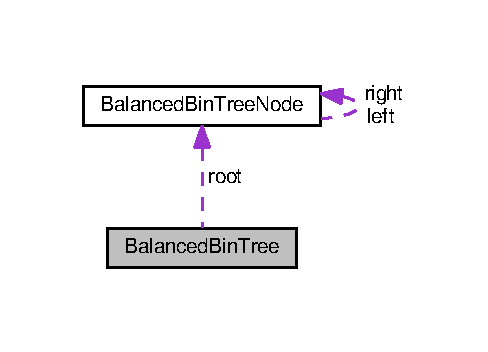
\includegraphics[width=234pt]{structBalancedBinTree__coll__graph}
\end{center}
\end{figure}
\subsection*{Public Attributes}
\begin{DoxyCompactItemize}
\item 
\mbox{\Hypertarget{structBalancedBinTree_a79eb6910645b1a28d977e59b69d89972}\label{structBalancedBinTree_a79eb6910645b1a28d977e59b69d89972}} 
\hyperlink{tree_8h_a2215a7c79686526cfed9198a82cb295e}{Tree\+Node} $\ast$ \hyperlink{structBalancedBinTree_a79eb6910645b1a28d977e59b69d89972}{root}
\begin{DoxyCompactList}\small\item\em pointer to generic data that is to be stored in the tree \end{DoxyCompactList}\item 
\mbox{\Hypertarget{structBalancedBinTree_a6ac05549d1e01bf3011ff1b772b1fc9b}\label{structBalancedBinTree_a6ac05549d1e01bf3011ff1b772b1fc9b}} 
int($\ast$ \hyperlink{structBalancedBinTree_a6ac05549d1e01bf3011ff1b772b1fc9b}{compare\+FP} )(void $\ast$data1, void $\ast$data2)
\begin{DoxyCompactList}\small\item\em function pointer to a comparison function for the purpose of inserting and deleting elements \end{DoxyCompactList}\item 
\mbox{\Hypertarget{structBalancedBinTree_a6f4f05cf895b0784475b307320c4f746}\label{structBalancedBinTree_a6f4f05cf895b0784475b307320c4f746}} 
void($\ast$ \hyperlink{structBalancedBinTree_a6f4f05cf895b0784475b307320c4f746}{destroy\+FP} )(void $\ast$data)
\begin{DoxyCompactList}\small\item\em function pointer to a function to free a single pointer that is deleted from the tree \end{DoxyCompactList}\item 
\mbox{\Hypertarget{structBalancedBinTree_a91f8d466e1dc38a603e2c85ec925d6e5}\label{structBalancedBinTree_a91f8d466e1dc38a603e2c85ec925d6e5}} 
void $\ast$($\ast$ \hyperlink{structBalancedBinTree_a91f8d466e1dc38a603e2c85ec925d6e5}{copy\+FP} )(void $\ast$to\+Be\+Copy)
\begin{DoxyCompactList}\small\item\em function pointer to a function that copies pointer data \end{DoxyCompactList}\end{DoxyCompactItemize}


The documentation for this struct was generated from the following file\+:\begin{DoxyCompactItemize}
\item 
include/\hyperlink{tree_8h}{tree.\+h}\end{DoxyCompactItemize}

\hypertarget{structBalancedBinTreeNode}{}\section{Balanced\+Bin\+Tree\+Node Struct Reference}
\label{structBalancedBinTreeNode}\index{Balanced\+Bin\+Tree\+Node@{Balanced\+Bin\+Tree\+Node}}


Collaboration diagram for Balanced\+Bin\+Tree\+Node\+:
\nopagebreak
\begin{figure}[H]
\begin{center}
\leavevmode
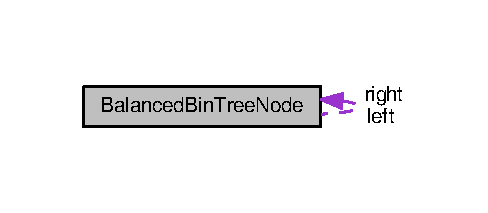
\includegraphics[width=234pt]{structBalancedBinTreeNode__coll__graph}
\end{center}
\end{figure}
\subsection*{Public Attributes}
\begin{DoxyCompactItemize}
\item 
\mbox{\Hypertarget{structBalancedBinTreeNode_a60ea906ce13bc63ec829be82d9fed633}\label{structBalancedBinTreeNode_a60ea906ce13bc63ec829be82d9fed633}} 
void $\ast$ \hyperlink{structBalancedBinTreeNode_a60ea906ce13bc63ec829be82d9fed633}{data}
\begin{DoxyCompactList}\small\item\em pointer to generic data that is to be stored in the heap \end{DoxyCompactList}\item 
\mbox{\Hypertarget{structBalancedBinTreeNode_a0cb8520a5b5b42c22472eaf5ea9084d7}\label{structBalancedBinTreeNode_a0cb8520a5b5b42c22472eaf5ea9084d7}} 
\hyperlink{tree_8h_a2215a7c79686526cfed9198a82cb295e}{Tree\+Node} $\ast$ \hyperlink{structBalancedBinTreeNode_a0cb8520a5b5b42c22472eaf5ea9084d7}{left}
\begin{DoxyCompactList}\small\item\em pointer to left tree node of current node. Null if empty. \end{DoxyCompactList}\item 
\mbox{\Hypertarget{structBalancedBinTreeNode_a6bb5c0f6c7098ba3b003846e8fc739ca}\label{structBalancedBinTreeNode_a6bb5c0f6c7098ba3b003846e8fc739ca}} 
\hyperlink{tree_8h_a2215a7c79686526cfed9198a82cb295e}{Tree\+Node} $\ast$ \hyperlink{structBalancedBinTreeNode_a6bb5c0f6c7098ba3b003846e8fc739ca}{right}
\begin{DoxyCompactList}\small\item\em pointer to right tree node of current node. Null if empty. \end{DoxyCompactList}\item 
\mbox{\Hypertarget{structBalancedBinTreeNode_acd64dda918a8d413103519903c6427ad}\label{structBalancedBinTreeNode_acd64dda918a8d413103519903c6427ad}} 
int {\bfseries height}
\end{DoxyCompactItemize}


The documentation for this struct was generated from the following file\+:\begin{DoxyCompactItemize}
\item 
include/\hyperlink{tree_8h}{tree.\+h}\end{DoxyCompactItemize}

\chapter{File Documentation}
\hypertarget{balancedTreeAPI_8h}{}\section{include/balanced\+Tree\+A\+PI.h File Reference}
\label{balancedTreeAPI_8h}\index{include/balanced\+Tree\+A\+P\+I.\+h@{include/balanced\+Tree\+A\+P\+I.\+h}}


File containing the functions that communicate with a self-\/balancing binary tree.  


{\ttfamily \#include $<$stdio.\+h$>$}\newline
{\ttfamily \#include $<$stdlib.\+h$>$}\newline
{\ttfamily \#include $<$string.\+h$>$}\newline
{\ttfamily \#include \char`\"{}tree.\+h\char`\"{}}\newline
Include dependency graph for balanced\+Tree\+A\+P\+I.\+h\+:
\nopagebreak
\begin{figure}[H]
\begin{center}
\leavevmode
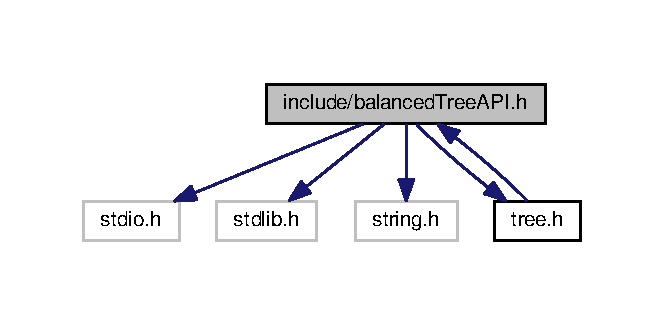
\includegraphics[width=319pt]{balancedTreeAPI_8h__incl}
\end{center}
\end{figure}
This graph shows which files directly or indirectly include this file\+:
\nopagebreak
\begin{figure}[H]
\begin{center}
\leavevmode
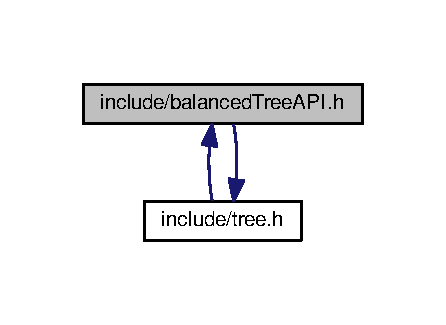
\includegraphics[width=214pt]{balancedTreeAPI_8h__dep__incl}
\end{center}
\end{figure}
\subsection*{Functions}
\begin{DoxyCompactItemize}
\item 
\hyperlink{tree_8h_afe8f5b9235f7a27460c81ff3ff48788e}{Tree} $\ast$ \hyperlink{balancedTreeAPI_8h_a54002b7e96754979d94eb4f3c5750328}{create\+Balanced\+Bin\+Tree} (int($\ast$compare\+FP)(void $\ast$data1, void $\ast$data2), void($\ast$destroy\+FP)(void $\ast$to\+Be\+Deleted), void $\ast$($\ast$copy\+FP)(void $\ast$to\+Be\+Copy))
\item 
\hyperlink{tree_8h_a2215a7c79686526cfed9198a82cb295e}{Tree\+Node} $\ast$ \hyperlink{balancedTreeAPI_8h_a59969ddb13215584df2a0df9816b5dbb}{create\+Balanced\+Bin\+Node} (void $\ast$data)
\item 
void \hyperlink{balancedTreeAPI_8h_a9a025a7c00f1f53f29b6184c25fb998d}{destroy\+Balanced\+Bin\+Tree} (\hyperlink{tree_8h_afe8f5b9235f7a27460c81ff3ff48788e}{Tree} $\ast$to\+Be\+Deleted)
\item 
void \hyperlink{balancedTreeAPI_8h_a8c90b112e2f12ffb017e386f92b69ac3}{tree\+Insert\+Node} (\hyperlink{tree_8h_afe8f5b9235f7a27460c81ff3ff48788e}{Tree} $\ast$the\+Tree, void $\ast$to\+Be\+Inserted)
\item 
void \hyperlink{balancedTreeAPI_8h_ab764e3af4d144b174b5db3adfe63a2c9}{tree\+Delete\+Node} (\hyperlink{tree_8h_afe8f5b9235f7a27460c81ff3ff48788e}{Tree} $\ast$the\+Tree, void $\ast$to\+Be\+Deleted)
\item 
int \hyperlink{balancedTreeAPI_8h_a59f1af69a351e89867db66987a0666e0}{tree\+Is\+Empty} (\hyperlink{tree_8h_afe8f5b9235f7a27460c81ff3ff48788e}{Tree} $\ast$the\+Tree)
\item 
int \hyperlink{balancedTreeAPI_8h_aff810699a02179aeabe9d5ab799dc766}{tree\+Has\+Two\+Children} (\hyperlink{tree_8h_a2215a7c79686526cfed9198a82cb295e}{Tree\+Node} $\ast$root)
\item 
void $\ast$ \hyperlink{balancedTreeAPI_8h_acccfb57183ab643ecb0f4a22f33d9b65}{tree\+Find\+Node} (\hyperlink{tree_8h_afe8f5b9235f7a27460c81ff3ff48788e}{Tree} $\ast$the\+Tree, void $\ast$data)
\item 
void $\ast$ \hyperlink{balancedTreeAPI_8h_a3bdbbebdedf6e4a4b782b79e8da849fe}{tree\+Find\+Min} (\hyperlink{tree_8h_afe8f5b9235f7a27460c81ff3ff48788e}{Tree} $\ast$the\+Tree)
\item 
void $\ast$ \hyperlink{balancedTreeAPI_8h_aa60a5fd0f6e263bc2ad8be9a83675ce1}{tree\+Find\+Max} (\hyperlink{tree_8h_afe8f5b9235f7a27460c81ff3ff48788e}{Tree} $\ast$the\+Tree)
\item 
void \hyperlink{balancedTreeAPI_8h_a46434e742f064d38f81b38924101ab2d}{tree\+In\+Order\+Print} (\hyperlink{tree_8h_afe8f5b9235f7a27460c81ff3ff48788e}{Tree} $\ast$the\+Tree, void($\ast$print\+Node\+FP)(void $\ast$data))
\item 
void \hyperlink{balancedTreeAPI_8h_a016871075d74c03a9a7a9e1a1b9b786c}{tree\+Pre\+Order\+Print} (\hyperlink{tree_8h_afe8f5b9235f7a27460c81ff3ff48788e}{Tree} $\ast$the\+Tree, void($\ast$print\+Node\+FP)(void $\ast$data))
\item 
void \hyperlink{balancedTreeAPI_8h_a6c42e5d760518c090eb6eb8b9bff62f8}{tree\+Post\+Order\+Print} (\hyperlink{tree_8h_afe8f5b9235f7a27460c81ff3ff48788e}{Tree} $\ast$the\+Tree, void($\ast$print\+Node\+FP)(void $\ast$data))
\end{DoxyCompactItemize}


\subsection{Detailed Description}
File containing the functions that communicate with a self-\/balancing binary tree. 

\begin{DoxyAuthor}{Author}
Michael Ellis 
\end{DoxyAuthor}
\begin{DoxyDate}{Date}
April 2017 
\end{DoxyDate}


\subsection{Function Documentation}
\mbox{\Hypertarget{balancedTreeAPI_8h_a59969ddb13215584df2a0df9816b5dbb}\label{balancedTreeAPI_8h_a59969ddb13215584df2a0df9816b5dbb}} 
\index{balanced\+Tree\+A\+P\+I.\+h@{balanced\+Tree\+A\+P\+I.\+h}!create\+Balanced\+Bin\+Node@{create\+Balanced\+Bin\+Node}}
\index{create\+Balanced\+Bin\+Node@{create\+Balanced\+Bin\+Node}!balanced\+Tree\+A\+P\+I.\+h@{balanced\+Tree\+A\+P\+I.\+h}}
\subsubsection{\texorpdfstring{create\+Balanced\+Bin\+Node()}{createBalancedBinNode()}}
{\footnotesize\ttfamily \hyperlink{tree_8h_a2215a7c79686526cfed9198a82cb295e}{Tree\+Node}$\ast$ create\+Balanced\+Bin\+Node (\begin{DoxyParamCaption}\item[{void $\ast$}]{data }\end{DoxyParamCaption})}

This function creates a tree node for a self-\/balancing binary tree. 
\begin{DoxyParams}{Parameters}
{\em data} & pointer to data that is to be added to a self-\/balancing binary tree. \\
\hline
\end{DoxyParams}
\mbox{\Hypertarget{balancedTreeAPI_8h_a54002b7e96754979d94eb4f3c5750328}\label{balancedTreeAPI_8h_a54002b7e96754979d94eb4f3c5750328}} 
\index{balanced\+Tree\+A\+P\+I.\+h@{balanced\+Tree\+A\+P\+I.\+h}!create\+Balanced\+Bin\+Tree@{create\+Balanced\+Bin\+Tree}}
\index{create\+Balanced\+Bin\+Tree@{create\+Balanced\+Bin\+Tree}!balanced\+Tree\+A\+P\+I.\+h@{balanced\+Tree\+A\+P\+I.\+h}}
\subsubsection{\texorpdfstring{create\+Balanced\+Bin\+Tree()}{createBalancedBinTree()}}
{\footnotesize\ttfamily \hyperlink{tree_8h_afe8f5b9235f7a27460c81ff3ff48788e}{Tree}$\ast$ create\+Balanced\+Bin\+Tree (\begin{DoxyParamCaption}\item[{int($\ast$)(void $\ast$data1, void $\ast$data2)}]{compare\+FP,  }\item[{void($\ast$)(void $\ast$to\+Be\+Deleted)}]{destroy\+FP,  }\item[{void $\ast$($\ast$)(void $\ast$to\+Be\+Copy)}]{copy\+FP }\end{DoxyParamCaption})}

This function returns a pointer to a binary tree. You must send pointers to the compare and destroy functions when you create the tree. 
\begin{DoxyParams}{Parameters}
{\em compare\+FP} & function pointer to allow for comparison between two generic data types \\
\hline
{\em destroy\+FP} & function pointer to allow for pointer deletion. \\
\hline
{\em copy\+FP} & function pointer to a function that copies pointer data to a new pointer. \\
\hline
\end{DoxyParams}
\begin{DoxyReturn}{Returns}
If successful, returns a pointer to a binary tree. Returns null if the memory allocation fails. 
\end{DoxyReturn}
\mbox{\Hypertarget{balancedTreeAPI_8h_a9a025a7c00f1f53f29b6184c25fb998d}\label{balancedTreeAPI_8h_a9a025a7c00f1f53f29b6184c25fb998d}} 
\index{balanced\+Tree\+A\+P\+I.\+h@{balanced\+Tree\+A\+P\+I.\+h}!destroy\+Balanced\+Bin\+Tree@{destroy\+Balanced\+Bin\+Tree}}
\index{destroy\+Balanced\+Bin\+Tree@{destroy\+Balanced\+Bin\+Tree}!balanced\+Tree\+A\+P\+I.\+h@{balanced\+Tree\+A\+P\+I.\+h}}
\subsubsection{\texorpdfstring{destroy\+Balanced\+Bin\+Tree()}{destroyBalancedBinTree()}}
{\footnotesize\ttfamily void destroy\+Balanced\+Bin\+Tree (\begin{DoxyParamCaption}\item[{\hyperlink{tree_8h_afe8f5b9235f7a27460c81ff3ff48788e}{Tree} $\ast$}]{to\+Be\+Deleted }\end{DoxyParamCaption})}

This function destroys a binary tree and all data that is in the tree when destroy is called. 
\begin{DoxyParams}{Parameters}
{\em to\+Be\+Deleted} & pointer to binary tree created via create\+Balanced\+Bin\+Tree \\
\hline
\end{DoxyParams}
\mbox{\Hypertarget{balancedTreeAPI_8h_ab764e3af4d144b174b5db3adfe63a2c9}\label{balancedTreeAPI_8h_ab764e3af4d144b174b5db3adfe63a2c9}} 
\index{balanced\+Tree\+A\+P\+I.\+h@{balanced\+Tree\+A\+P\+I.\+h}!tree\+Delete\+Node@{tree\+Delete\+Node}}
\index{tree\+Delete\+Node@{tree\+Delete\+Node}!balanced\+Tree\+A\+P\+I.\+h@{balanced\+Tree\+A\+P\+I.\+h}}
\subsubsection{\texorpdfstring{tree\+Delete\+Node()}{treeDeleteNode()}}
{\footnotesize\ttfamily void tree\+Delete\+Node (\begin{DoxyParamCaption}\item[{\hyperlink{tree_8h_afe8f5b9235f7a27460c81ff3ff48788e}{Tree} $\ast$}]{the\+Tree,  }\item[{void $\ast$}]{to\+Be\+Deleted }\end{DoxyParamCaption})}

Function to delete a node from a self-\/balancing binary tree. 
\begin{DoxyParams}{Parameters}
{\em the\+Tree} & pointer to a self-\/balancing binary tree \\
\hline
{\em to\+Be\+Deleted} & pointer to generic data that is to be deleted from the self-\/balancing binary tree \\
\hline
\end{DoxyParams}
\mbox{\Hypertarget{balancedTreeAPI_8h_aa60a5fd0f6e263bc2ad8be9a83675ce1}\label{balancedTreeAPI_8h_aa60a5fd0f6e263bc2ad8be9a83675ce1}} 
\index{balanced\+Tree\+A\+P\+I.\+h@{balanced\+Tree\+A\+P\+I.\+h}!tree\+Find\+Max@{tree\+Find\+Max}}
\index{tree\+Find\+Max@{tree\+Find\+Max}!balanced\+Tree\+A\+P\+I.\+h@{balanced\+Tree\+A\+P\+I.\+h}}
\subsubsection{\texorpdfstring{tree\+Find\+Max()}{treeFindMax()}}
{\footnotesize\ttfamily void$\ast$ tree\+Find\+Max (\begin{DoxyParamCaption}\item[{\hyperlink{tree_8h_afe8f5b9235f7a27460c81ff3ff48788e}{Tree} $\ast$}]{the\+Tree }\end{DoxyParamCaption})}

Function to return the largest value of a tree, dependant on the compare function pointer parameters. 
\begin{DoxyParams}{Parameters}
{\em the\+Tree} & pointer to a self-\/balancing binary tree\textquotesingle{}s root \\
\hline
\end{DoxyParams}
\begin{DoxyReturn}{Returns}
pointer to the maximum value found. If tree is empty, return N\+U\+LL. 
\end{DoxyReturn}
\mbox{\Hypertarget{balancedTreeAPI_8h_a3bdbbebdedf6e4a4b782b79e8da849fe}\label{balancedTreeAPI_8h_a3bdbbebdedf6e4a4b782b79e8da849fe}} 
\index{balanced\+Tree\+A\+P\+I.\+h@{balanced\+Tree\+A\+P\+I.\+h}!tree\+Find\+Min@{tree\+Find\+Min}}
\index{tree\+Find\+Min@{tree\+Find\+Min}!balanced\+Tree\+A\+P\+I.\+h@{balanced\+Tree\+A\+P\+I.\+h}}
\subsubsection{\texorpdfstring{tree\+Find\+Min()}{treeFindMin()}}
{\footnotesize\ttfamily void$\ast$ tree\+Find\+Min (\begin{DoxyParamCaption}\item[{\hyperlink{tree_8h_afe8f5b9235f7a27460c81ff3ff48788e}{Tree} $\ast$}]{the\+Tree }\end{DoxyParamCaption})}

Function to return the smallest value of a tree, dependant on the compare function pointer parameters. 
\begin{DoxyParams}{Parameters}
{\em the\+Tree} & pointer to a self-\/balancing binary tree\textquotesingle{}s root \\
\hline
\end{DoxyParams}
\begin{DoxyReturn}{Returns}
pointer to the min found. If tree is empty, return N\+U\+LL. 
\end{DoxyReturn}
\mbox{\Hypertarget{balancedTreeAPI_8h_acccfb57183ab643ecb0f4a22f33d9b65}\label{balancedTreeAPI_8h_acccfb57183ab643ecb0f4a22f33d9b65}} 
\index{balanced\+Tree\+A\+P\+I.\+h@{balanced\+Tree\+A\+P\+I.\+h}!tree\+Find\+Node@{tree\+Find\+Node}}
\index{tree\+Find\+Node@{tree\+Find\+Node}!balanced\+Tree\+A\+P\+I.\+h@{balanced\+Tree\+A\+P\+I.\+h}}
\subsubsection{\texorpdfstring{tree\+Find\+Node()}{treeFindNode()}}
{\footnotesize\ttfamily void$\ast$ tree\+Find\+Node (\begin{DoxyParamCaption}\item[{\hyperlink{tree_8h_afe8f5b9235f7a27460c81ff3ff48788e}{Tree} $\ast$}]{the\+Tree,  }\item[{void $\ast$}]{data }\end{DoxyParamCaption})}

Function to return a given value in the tree, dependant on the compare function pointer parameters. Compares nodes, until compare function returns zero, or the tree is exhausted. 
\begin{DoxyParams}{Parameters}
{\em the\+Tree} & pointer to a self-\/balancing binary tree\textquotesingle{}s root \\
\hline
\end{DoxyParams}
\begin{DoxyReturn}{Returns}
pointer to the data found. If tree is empty or data is not found, return N\+U\+LL. 
\end{DoxyReturn}
\mbox{\Hypertarget{balancedTreeAPI_8h_aff810699a02179aeabe9d5ab799dc766}\label{balancedTreeAPI_8h_aff810699a02179aeabe9d5ab799dc766}} 
\index{balanced\+Tree\+A\+P\+I.\+h@{balanced\+Tree\+A\+P\+I.\+h}!tree\+Has\+Two\+Children@{tree\+Has\+Two\+Children}}
\index{tree\+Has\+Two\+Children@{tree\+Has\+Two\+Children}!balanced\+Tree\+A\+P\+I.\+h@{balanced\+Tree\+A\+P\+I.\+h}}
\subsubsection{\texorpdfstring{tree\+Has\+Two\+Children()}{treeHasTwoChildren()}}
{\footnotesize\ttfamily int tree\+Has\+Two\+Children (\begin{DoxyParamCaption}\item[{\hyperlink{tree_8h_a2215a7c79686526cfed9198a82cb295e}{Tree\+Node} $\ast$}]{root }\end{DoxyParamCaption})}

Function to determine if a binary tree node has two children. 
\begin{DoxyParams}{Parameters}
{\em root} & pointer to a self-\/balancing binary tree\textquotesingle{}s root \\
\hline
\end{DoxyParams}
\begin{DoxyReturn}{Returns}
If tree is empty, or does not exist, return 1. Otherwise, return 0. 
\end{DoxyReturn}
\mbox{\Hypertarget{balancedTreeAPI_8h_a46434e742f064d38f81b38924101ab2d}\label{balancedTreeAPI_8h_a46434e742f064d38f81b38924101ab2d}} 
\index{balanced\+Tree\+A\+P\+I.\+h@{balanced\+Tree\+A\+P\+I.\+h}!tree\+In\+Order\+Print@{tree\+In\+Order\+Print}}
\index{tree\+In\+Order\+Print@{tree\+In\+Order\+Print}!balanced\+Tree\+A\+P\+I.\+h@{balanced\+Tree\+A\+P\+I.\+h}}
\subsubsection{\texorpdfstring{tree\+In\+Order\+Print()}{treeInOrderPrint()}}
{\footnotesize\ttfamily void tree\+In\+Order\+Print (\begin{DoxyParamCaption}\item[{\hyperlink{tree_8h_afe8f5b9235f7a27460c81ff3ff48788e}{Tree} $\ast$}]{the\+Tree,  }\item[{void($\ast$)(void $\ast$data)}]{print\+Node\+FP }\end{DoxyParamCaption})}

function to print a tree in-\/order. EG A / \textbackslash{} B C / \textbackslash{} / \textbackslash{} D F G E would print nodes thusly\+: D-\/$>$B-\/$>$F-\/$>$A-\/$>$G-\/$>$C-\/$>$E 
\begin{DoxyParams}{Parameters}
{\em the\+Tree} & pointer to a self-\/balancing binary tree \\
\hline
{\em print\+Node\+FP} & pointer to a function to print void pointer data. \\
\hline
\end{DoxyParams}
\mbox{\Hypertarget{balancedTreeAPI_8h_a8c90b112e2f12ffb017e386f92b69ac3}\label{balancedTreeAPI_8h_a8c90b112e2f12ffb017e386f92b69ac3}} 
\index{balanced\+Tree\+A\+P\+I.\+h@{balanced\+Tree\+A\+P\+I.\+h}!tree\+Insert\+Node@{tree\+Insert\+Node}}
\index{tree\+Insert\+Node@{tree\+Insert\+Node}!balanced\+Tree\+A\+P\+I.\+h@{balanced\+Tree\+A\+P\+I.\+h}}
\subsubsection{\texorpdfstring{tree\+Insert\+Node()}{treeInsertNode()}}
{\footnotesize\ttfamily void tree\+Insert\+Node (\begin{DoxyParamCaption}\item[{\hyperlink{tree_8h_afe8f5b9235f7a27460c81ff3ff48788e}{Tree} $\ast$}]{the\+Tree,  }\item[{void $\ast$}]{to\+Be\+Inserted }\end{DoxyParamCaption})}

Function to insert a node into a self-\/balancing binary tree. 
\begin{DoxyParams}{Parameters}
{\em the\+Tree} & pointer to a self-\/balancing binary tree \\
\hline
{\em to\+Be\+Inserted} & pointer to generic data that is to be inserted into the self-\/balancing binary tree \\
\hline
\end{DoxyParams}
\mbox{\Hypertarget{balancedTreeAPI_8h_a59f1af69a351e89867db66987a0666e0}\label{balancedTreeAPI_8h_a59f1af69a351e89867db66987a0666e0}} 
\index{balanced\+Tree\+A\+P\+I.\+h@{balanced\+Tree\+A\+P\+I.\+h}!tree\+Is\+Empty@{tree\+Is\+Empty}}
\index{tree\+Is\+Empty@{tree\+Is\+Empty}!balanced\+Tree\+A\+P\+I.\+h@{balanced\+Tree\+A\+P\+I.\+h}}
\subsubsection{\texorpdfstring{tree\+Is\+Empty()}{treeIsEmpty()}}
{\footnotesize\ttfamily int tree\+Is\+Empty (\begin{DoxyParamCaption}\item[{\hyperlink{tree_8h_afe8f5b9235f7a27460c81ff3ff48788e}{Tree} $\ast$}]{the\+Tree }\end{DoxyParamCaption})}

Function to determine if a binary tree is empty. 
\begin{DoxyParams}{Parameters}
{\em the\+Tree} & pointer to a self-\/balancing binary tree \\
\hline
\end{DoxyParams}
\begin{DoxyReturn}{Returns}
If tree is empty, return 1. Otherwise, return 0. 
\end{DoxyReturn}
\mbox{\Hypertarget{balancedTreeAPI_8h_a6c42e5d760518c090eb6eb8b9bff62f8}\label{balancedTreeAPI_8h_a6c42e5d760518c090eb6eb8b9bff62f8}} 
\index{balanced\+Tree\+A\+P\+I.\+h@{balanced\+Tree\+A\+P\+I.\+h}!tree\+Post\+Order\+Print@{tree\+Post\+Order\+Print}}
\index{tree\+Post\+Order\+Print@{tree\+Post\+Order\+Print}!balanced\+Tree\+A\+P\+I.\+h@{balanced\+Tree\+A\+P\+I.\+h}}
\subsubsection{\texorpdfstring{tree\+Post\+Order\+Print()}{treePostOrderPrint()}}
{\footnotesize\ttfamily void tree\+Post\+Order\+Print (\begin{DoxyParamCaption}\item[{\hyperlink{tree_8h_afe8f5b9235f7a27460c81ff3ff48788e}{Tree} $\ast$}]{the\+Tree,  }\item[{void($\ast$)(void $\ast$data)}]{print\+Node\+FP }\end{DoxyParamCaption})}

Function to print a tree in post-\/order. EG A / \textbackslash{} B C / \textbackslash{} / \textbackslash{} D F G E would print nodes thusly\+: D-\/$>$F-\/$>$B-\/$>$G-\/$>$C-\/$>$E-\/$>$A 
\begin{DoxyParams}{Parameters}
{\em the\+Tree} & pointer to a self-\/balancing binary tree\textquotesingle{}s root \\
\hline
{\em print\+Node\+FP} & pointer to a function to print void pointer data. \\
\hline
\end{DoxyParams}
\mbox{\Hypertarget{balancedTreeAPI_8h_a016871075d74c03a9a7a9e1a1b9b786c}\label{balancedTreeAPI_8h_a016871075d74c03a9a7a9e1a1b9b786c}} 
\index{balanced\+Tree\+A\+P\+I.\+h@{balanced\+Tree\+A\+P\+I.\+h}!tree\+Pre\+Order\+Print@{tree\+Pre\+Order\+Print}}
\index{tree\+Pre\+Order\+Print@{tree\+Pre\+Order\+Print}!balanced\+Tree\+A\+P\+I.\+h@{balanced\+Tree\+A\+P\+I.\+h}}
\subsubsection{\texorpdfstring{tree\+Pre\+Order\+Print()}{treePreOrderPrint()}}
{\footnotesize\ttfamily void tree\+Pre\+Order\+Print (\begin{DoxyParamCaption}\item[{\hyperlink{tree_8h_afe8f5b9235f7a27460c81ff3ff48788e}{Tree} $\ast$}]{the\+Tree,  }\item[{void($\ast$)(void $\ast$data)}]{print\+Node\+FP }\end{DoxyParamCaption})}

Function to print a tree pre-\/order. EG A / \textbackslash{} B C / \textbackslash{} / \textbackslash{} D F G E would print nodes thusly\+: A-\/$>$B-\/$>$D-\/$>$F-\/$>$C-\/$>$G-\/$>$E 
\begin{DoxyParams}{Parameters}
{\em the\+Tree} & pointer to a self-\/balancing binary tree \\
\hline
{\em print\+Node\+FP} & pointer to a function to print void pointer data. \\
\hline
\end{DoxyParams}

\hypertarget{tree_8h}{}\section{include/tree.h File Reference}
\label{tree_8h}\index{include/tree.\+h@{include/tree.\+h}}


File containing the structures for a self-\/balancing binary tree and additional functions.  


{\ttfamily \#include \char`\"{}balanced\+Tree\+A\+P\+I.\+h\char`\"{}}\newline
Include dependency graph for tree.\+h\+:
\nopagebreak
\begin{figure}[H]
\begin{center}
\leavevmode
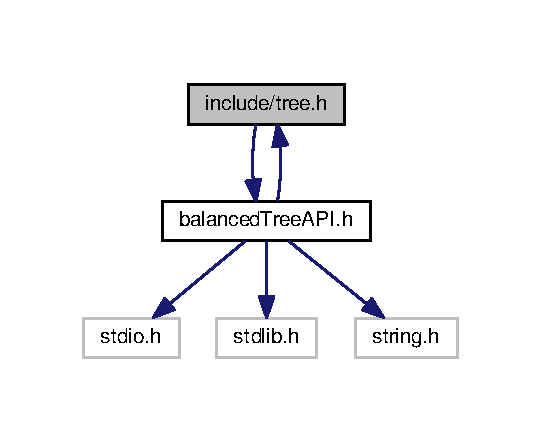
\includegraphics[width=260pt]{tree_8h__incl}
\end{center}
\end{figure}
This graph shows which files directly or indirectly include this file\+:
\nopagebreak
\begin{figure}[H]
\begin{center}
\leavevmode
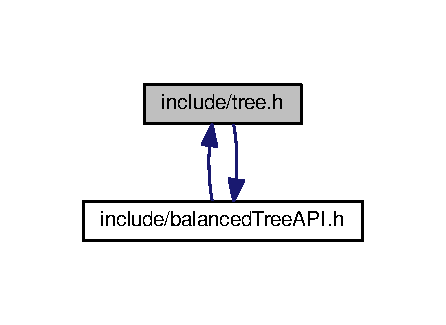
\includegraphics[width=214pt]{tree_8h__dep__incl}
\end{center}
\end{figure}
\subsection*{Classes}
\begin{DoxyCompactItemize}
\item 
struct \hyperlink{structBalancedBinTree}{Balanced\+Bin\+Tree}
\item 
struct \hyperlink{structBalancedBinTreeNode}{Balanced\+Bin\+Tree\+Node}
\end{DoxyCompactItemize}
\subsection*{Typedefs}
\begin{DoxyCompactItemize}
\item 
typedef struct \hyperlink{structBalancedBinTreeNode}{Balanced\+Bin\+Tree\+Node} \hyperlink{tree_8h_a2215a7c79686526cfed9198a82cb295e}{Tree\+Node}
\item 
typedef struct \hyperlink{structBalancedBinTree}{Balanced\+Bin\+Tree} \hyperlink{tree_8h_afe8f5b9235f7a27460c81ff3ff48788e}{Tree}
\end{DoxyCompactItemize}
\subsection*{Functions}
\begin{DoxyCompactItemize}
\item 
\hyperlink{tree_8h_a2215a7c79686526cfed9198a82cb295e}{Tree\+Node} $\ast$ \hyperlink{tree_8h_a637bee38441530e03b76fa0c98535a4b}{insert} (\hyperlink{tree_8h_a2215a7c79686526cfed9198a82cb295e}{Tree\+Node} $\ast$tree\+Root, void $\ast$data, int($\ast$compare\+FP)(void $\ast$data1, void $\ast$data2))
\item 
\hyperlink{tree_8h_a2215a7c79686526cfed9198a82cb295e}{Tree\+Node} $\ast$ \hyperlink{tree_8h_acb01f1169d0b166788b3dedd8c5108b0}{rotate\+With\+Left\+Child} (\hyperlink{tree_8h_a2215a7c79686526cfed9198a82cb295e}{Tree\+Node} $\ast$old\+Root)
\item 
\hyperlink{tree_8h_a2215a7c79686526cfed9198a82cb295e}{Tree\+Node} $\ast$ \hyperlink{tree_8h_a5453280718fc5133caff315b34abad20}{rotate\+With\+Right\+Child} (\hyperlink{tree_8h_a2215a7c79686526cfed9198a82cb295e}{Tree\+Node} $\ast$old\+Root)
\item 
\hyperlink{tree_8h_a2215a7c79686526cfed9198a82cb295e}{Tree\+Node} $\ast$ \hyperlink{tree_8h_a68e9e7b3bbc8b3535af3b9fc60bbbb22}{double\+Rotate\+With\+Right\+Child} (\hyperlink{tree_8h_a2215a7c79686526cfed9198a82cb295e}{Tree\+Node} $\ast$old\+Root)
\item 
\hyperlink{tree_8h_a2215a7c79686526cfed9198a82cb295e}{Tree\+Node} $\ast$ \hyperlink{tree_8h_a35f01c890aaa69ce4751decfd2944ab3}{double\+Rotate\+With\+Left\+Child} (\hyperlink{tree_8h_a2215a7c79686526cfed9198a82cb295e}{Tree\+Node} $\ast$old\+Root)
\item 
\hyperlink{tree_8h_a2215a7c79686526cfed9198a82cb295e}{Tree\+Node} $\ast$ \hyperlink{tree_8h_ad3f2d9b1b5412380074254b09dbddc71}{delete} (\hyperlink{tree_8h_a2215a7c79686526cfed9198a82cb295e}{Tree\+Node} $\ast$root, void $\ast$data, \hyperlink{tree_8h_afe8f5b9235f7a27460c81ff3ff48788e}{Tree} $\ast$the\+Tree)
\end{DoxyCompactItemize}


\subsection{Detailed Description}
File containing the structures for a self-\/balancing binary tree and additional functions. 

\begin{DoxyDate}{Date}
July 2018 
\end{DoxyDate}


\subsection{Typedef Documentation}
\mbox{\Hypertarget{tree_8h_afe8f5b9235f7a27460c81ff3ff48788e}\label{tree_8h_afe8f5b9235f7a27460c81ff3ff48788e}} 
\index{tree.\+h@{tree.\+h}!Tree@{Tree}}
\index{Tree@{Tree}!tree.\+h@{tree.\+h}}
\subsubsection{\texorpdfstring{Tree}{Tree}}
{\footnotesize\ttfamily typedef struct \hyperlink{structBalancedBinTree}{Balanced\+Bin\+Tree} \hyperlink{tree_8h_afe8f5b9235f7a27460c81ff3ff48788e}{Tree}}

typedef for struct name \mbox{\Hypertarget{tree_8h_a2215a7c79686526cfed9198a82cb295e}\label{tree_8h_a2215a7c79686526cfed9198a82cb295e}} 
\index{tree.\+h@{tree.\+h}!Tree\+Node@{Tree\+Node}}
\index{Tree\+Node@{Tree\+Node}!tree.\+h@{tree.\+h}}
\subsubsection{\texorpdfstring{Tree\+Node}{TreeNode}}
{\footnotesize\ttfamily typedef struct \hyperlink{structBalancedBinTreeNode}{Balanced\+Bin\+Tree\+Node} \hyperlink{tree_8h_a2215a7c79686526cfed9198a82cb295e}{Tree\+Node}}

typedef for struct name 

\subsection{Function Documentation}
\mbox{\Hypertarget{tree_8h_ad3f2d9b1b5412380074254b09dbddc71}\label{tree_8h_ad3f2d9b1b5412380074254b09dbddc71}} 
\index{tree.\+h@{tree.\+h}!delete@{delete}}
\index{delete@{delete}!tree.\+h@{tree.\+h}}
\subsubsection{\texorpdfstring{delete()}{delete()}}
{\footnotesize\ttfamily \hyperlink{tree_8h_a2215a7c79686526cfed9198a82cb295e}{Tree\+Node}$\ast$ delete (\begin{DoxyParamCaption}\item[{\hyperlink{tree_8h_a2215a7c79686526cfed9198a82cb295e}{Tree\+Node} $\ast$}]{root,  }\item[{void $\ast$}]{data,  }\item[{\hyperlink{tree_8h_afe8f5b9235f7a27460c81ff3ff48788e}{Tree} $\ast$}]{the\+Tree }\end{DoxyParamCaption})}

Function to delete a node 
\begin{DoxyParams}{Parameters}
{\em root} & pointer to root of subtree \\
\hline
{\em data} & data that should be deleted \\
\hline
{\em the\+Tree} & pointer to entire tree \\
\hline
\end{DoxyParams}
\mbox{\Hypertarget{tree_8h_a35f01c890aaa69ce4751decfd2944ab3}\label{tree_8h_a35f01c890aaa69ce4751decfd2944ab3}} 
\index{tree.\+h@{tree.\+h}!double\+Rotate\+With\+Left\+Child@{double\+Rotate\+With\+Left\+Child}}
\index{double\+Rotate\+With\+Left\+Child@{double\+Rotate\+With\+Left\+Child}!tree.\+h@{tree.\+h}}
\subsubsection{\texorpdfstring{double\+Rotate\+With\+Left\+Child()}{doubleRotateWithLeftChild()}}
{\footnotesize\ttfamily \hyperlink{tree_8h_a2215a7c79686526cfed9198a82cb295e}{Tree\+Node}$\ast$ double\+Rotate\+With\+Left\+Child (\begin{DoxyParamCaption}\item[{\hyperlink{tree_8h_a2215a7c79686526cfed9198a82cb295e}{Tree\+Node} $\ast$}]{old\+Root }\end{DoxyParamCaption})}

Function to complete double rotatatoion with left child 
\begin{DoxyParams}{Parameters}
{\em oldroot} & pointer to original subtree root \\
\hline
\end{DoxyParams}
\begin{DoxyReturn}{Returns}
pointer to child 
\end{DoxyReturn}
\mbox{\Hypertarget{tree_8h_a68e9e7b3bbc8b3535af3b9fc60bbbb22}\label{tree_8h_a68e9e7b3bbc8b3535af3b9fc60bbbb22}} 
\index{tree.\+h@{tree.\+h}!double\+Rotate\+With\+Right\+Child@{double\+Rotate\+With\+Right\+Child}}
\index{double\+Rotate\+With\+Right\+Child@{double\+Rotate\+With\+Right\+Child}!tree.\+h@{tree.\+h}}
\subsubsection{\texorpdfstring{double\+Rotate\+With\+Right\+Child()}{doubleRotateWithRightChild()}}
{\footnotesize\ttfamily \hyperlink{tree_8h_a2215a7c79686526cfed9198a82cb295e}{Tree\+Node}$\ast$ double\+Rotate\+With\+Right\+Child (\begin{DoxyParamCaption}\item[{\hyperlink{tree_8h_a2215a7c79686526cfed9198a82cb295e}{Tree\+Node} $\ast$}]{old\+Root }\end{DoxyParamCaption})}

Function to complete double rotatatoion with right child 
\begin{DoxyParams}{Parameters}
{\em oldroot} & pointer to original subtree root \\
\hline
\end{DoxyParams}
\begin{DoxyReturn}{Returns}
pointer to child 
\end{DoxyReturn}
\mbox{\Hypertarget{tree_8h_a637bee38441530e03b76fa0c98535a4b}\label{tree_8h_a637bee38441530e03b76fa0c98535a4b}} 
\index{tree.\+h@{tree.\+h}!insert@{insert}}
\index{insert@{insert}!tree.\+h@{tree.\+h}}
\subsubsection{\texorpdfstring{insert()}{insert()}}
{\footnotesize\ttfamily \hyperlink{tree_8h_a2215a7c79686526cfed9198a82cb295e}{Tree\+Node}$\ast$ insert (\begin{DoxyParamCaption}\item[{\hyperlink{tree_8h_a2215a7c79686526cfed9198a82cb295e}{Tree\+Node} $\ast$}]{tree\+Root,  }\item[{void $\ast$}]{data,  }\item[{int($\ast$)(void $\ast$data1, void $\ast$data2)}]{compare\+FP }\end{DoxyParamCaption})}

Function to insert data into the tree 
\begin{DoxyParams}{Parameters}
{\em tree\+Root} & pointer to tree or subtree root \\
\hline
{\em data} & pointer to void data type \\
\hline
{\em compare\+FP} & pointer to compare function \\
\hline
\end{DoxyParams}
\begin{DoxyReturn}{Returns}
pointer to inserted node 
\end{DoxyReturn}
\mbox{\Hypertarget{tree_8h_acb01f1169d0b166788b3dedd8c5108b0}\label{tree_8h_acb01f1169d0b166788b3dedd8c5108b0}} 
\index{tree.\+h@{tree.\+h}!rotate\+With\+Left\+Child@{rotate\+With\+Left\+Child}}
\index{rotate\+With\+Left\+Child@{rotate\+With\+Left\+Child}!tree.\+h@{tree.\+h}}
\subsubsection{\texorpdfstring{rotate\+With\+Left\+Child()}{rotateWithLeftChild()}}
{\footnotesize\ttfamily \hyperlink{tree_8h_a2215a7c79686526cfed9198a82cb295e}{Tree\+Node}$\ast$ rotate\+With\+Left\+Child (\begin{DoxyParamCaption}\item[{\hyperlink{tree_8h_a2215a7c79686526cfed9198a82cb295e}{Tree\+Node} $\ast$}]{old\+Root }\end{DoxyParamCaption})}

Function to rotate with left child 
\begin{DoxyParams}{Parameters}
{\em oldroot} & pointer to original subtree root \\
\hline
\end{DoxyParams}
\begin{DoxyReturn}{Returns}
pointer to child 
\end{DoxyReturn}
\mbox{\Hypertarget{tree_8h_a5453280718fc5133caff315b34abad20}\label{tree_8h_a5453280718fc5133caff315b34abad20}} 
\index{tree.\+h@{tree.\+h}!rotate\+With\+Right\+Child@{rotate\+With\+Right\+Child}}
\index{rotate\+With\+Right\+Child@{rotate\+With\+Right\+Child}!tree.\+h@{tree.\+h}}
\subsubsection{\texorpdfstring{rotate\+With\+Right\+Child()}{rotateWithRightChild()}}
{\footnotesize\ttfamily \hyperlink{tree_8h_a2215a7c79686526cfed9198a82cb295e}{Tree\+Node}$\ast$ rotate\+With\+Right\+Child (\begin{DoxyParamCaption}\item[{\hyperlink{tree_8h_a2215a7c79686526cfed9198a82cb295e}{Tree\+Node} $\ast$}]{old\+Root }\end{DoxyParamCaption})}

Function to rotate with right child 
\begin{DoxyParams}{Parameters}
{\em oldroot} & pointer to original subtree root \\
\hline
\end{DoxyParams}
\begin{DoxyReturn}{Returns}
pointer to child 
\end{DoxyReturn}

%--- End generated contents ---

% Index
\backmatter
\newpage
\phantomsection
\clearemptydoublepage
\addcontentsline{toc}{chapter}{Index}
\printindex

\end{document}
